\documentclass{amsart}

\usepackage{tikz}
\usepackage{tikz-3dplot}
\usetikzlibrary{matrix}
\usetikzlibrary{positioning}
\usetikzlibrary{fit}


\usepackage{linear_alg}

\begin{document}

\begin{center}
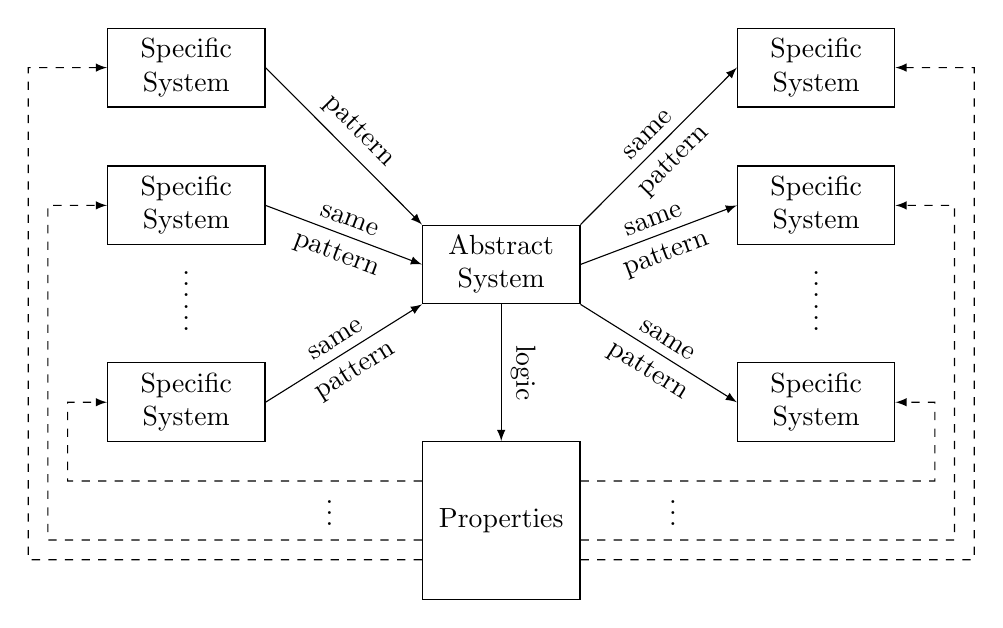
\begin{tikzpicture}[
	point/.style={circle,draw,very thin,fill,inner sep=0pt,minimum size=4pt},
	vector/.style={-latex},
]

	% center boxes
	\node[draw, fit={(0,0) (2,1)}, inner sep=0pt, label={[align=center]center:Abstract\\System}] (AS) {};
	\node[
		draw, yshift=-3.75cm,
		fit={(0,0) (2,2)}, inner sep=0pt,
		label=center:Properties
	] (P) {};
	\draw[vector] (AS.south) to node[sloped,above] {logic} (P.north);

	% LHS boxes
	\node[
		draw, xshift=-4cm, yshift=2.5cm,
		fit={(0,0) (2,1)}, inner sep=0pt,
		label={[align=center]center:Specific\\System}
	] (SS1) {};
	\draw[vector] (SS1.east) to node[sloped,above] {pattern} (AS.north west);

	\node[
		draw, xshift=-4cm, yshift=0.75cm,
		fit={(0,0) (2,1)}, inner sep=0pt,
		label={[align=center]center:Specific\\System}
	] (SS2) {};
	\draw[vector] (SS2.east) to node[sloped,above] {same} node[sloped,below] {pattern} (AS.west);

	\node[
		draw, xshift=-4cm, yshift=-1.75cm,
		fit={(0,0) (2,1)}, inner sep=0pt,
		label={[align=center]center:Specific\\System}
	] (SS3) {};
	\draw[vector] (SS3.east) to node[sloped,above] {same} node[sloped,below] {pattern} (AS.south west);

	\node[below=of SS2, yshift=1cm] (vdot) {$\vdots$};
	\node[below=of vdot, yshift=1.35cm] {$\vdots$};

	\draw[vector,dashed]
		([yshift=0.5cm] P.west) to
		([xshift=-0.5cm,yshift=-1cm] SS3.west) to
		([xshift=-0.5cm] SS3.west) to
		(SS3.west);

	\node[left=of P,yshift=0.2cm] {$\vdots$};

	\draw[vector,dashed]
		([yshift=-0.25cm] P.west) to
		([xshift=-0.75cm,yshift=-4.25cm] SS2.west) to
		([xshift=-0.75cm] SS2.west) to
		(SS2.west);

	\draw[vector,dashed]
		([yshift=-0.5cm] P.west) to
		([xshift=-1cm,yshift=-6.25cm] SS1.west) to
		([xshift=-1cm] SS1.west) to
		(SS1.west);

	% RHS boxes
	\node[
		draw, xshift=4cm, yshift=2.5cm,
		fit={(0,0) (2,1)}, inner sep=0pt,
		label={[align=center]center:Specific\\System}
	] (SS1) {};
	\draw[vector] (AS.north east) to node[sloped,above] {same} node[sloped,below] {pattern} (SS1.west);

	\node[
		draw, xshift=4cm, yshift=0.75cm,
		fit={(0,0) (2,1)}, inner sep=0pt,
		label={[align=center]center:Specific\\System}
	] (SS2) {};
	\draw[vector] (AS.east) to node[sloped,above] {same} node[sloped,below] {pattern} (SS2.west);

	\node[
		draw, xshift=4cm, yshift=-1.75cm,
		fit={(0,0) (2,1)}, inner sep=0pt,
		label={[align=center]center:Specific\\System}
	] (SS3) {};
	\draw[vector] (AS.south east) to node[sloped,above] {same} node[sloped,below] {pattern} (SS3.west);

	\node[below=of SS2, yshift=1cm] (vdot) {$\vdots$};
	\node[below=of vdot, yshift=1.35cm] {$\vdots$};

	\draw[vector,dashed]
		([yshift=0.5cm] P.east) to
		([xshift=0.5cm,yshift=-1cm] SS3.east) to
		([xshift=0.5cm] SS3.east) to
		(SS3.east);

	\node[right=of P,yshift=0.2cm] {$\vdots$};

	\draw[vector,dashed]
		([yshift=-0.25cm] P.east) to
		([xshift=0.75cm,yshift=-4.25cm] SS2.east) to
		([xshift=0.75cm] SS2.east) to
		(SS2.east);

	\draw[vector,dashed]
		([yshift=-0.5cm] P.east) to
		([xshift=1cm,yshift=-6.25cm] SS1.east) to
		([xshift=1cm] SS1.east) to
		(SS1.east);

\end{tikzpicture}
\end{center}

%\[
%	\left\lvert\begin{array}{rrrr}
%			1 & -1 & 2 & 1 \\
%			2 & 0 & 1 & 1 \\
%			0 & 1 & 0 & -3 \\
%			1 & -2 & -1 & 0 \\
%	 \end{array}\right\rvert
%\]



\end{document}
